\documentclass[12pt]{article}
\oddsidemargin=-0.250in
\evensidemargin=0.0in
\textwidth=6.75in
\topmargin=-.35in
\textheight=9in
\usepackage{graphicx}
 
\begin{document}
\pagestyle{empty}

\begin{center}
{\Large {\bf Planes}}\\
\medskip
{\large {Calculus III}}\\
\medskip
College of the Atlantic\\
\end{center}
\smallskip

\begin{enumerate}


\item Suppose a plane has a $z$-intercept of $7$, a slope of $-3$ in
the $x$ direction and a slope of $2$ in the $y$ direction.  
\begin{enumerate}
  \item If you start at the origin and walk to the point $(x,y) =
    (3,5)$, what is your $z$-value? 
  \item What is the equation of this plane?
\end{enumerate}

\begin{figure}[h]
\begin{center}
\vspace{0mm}
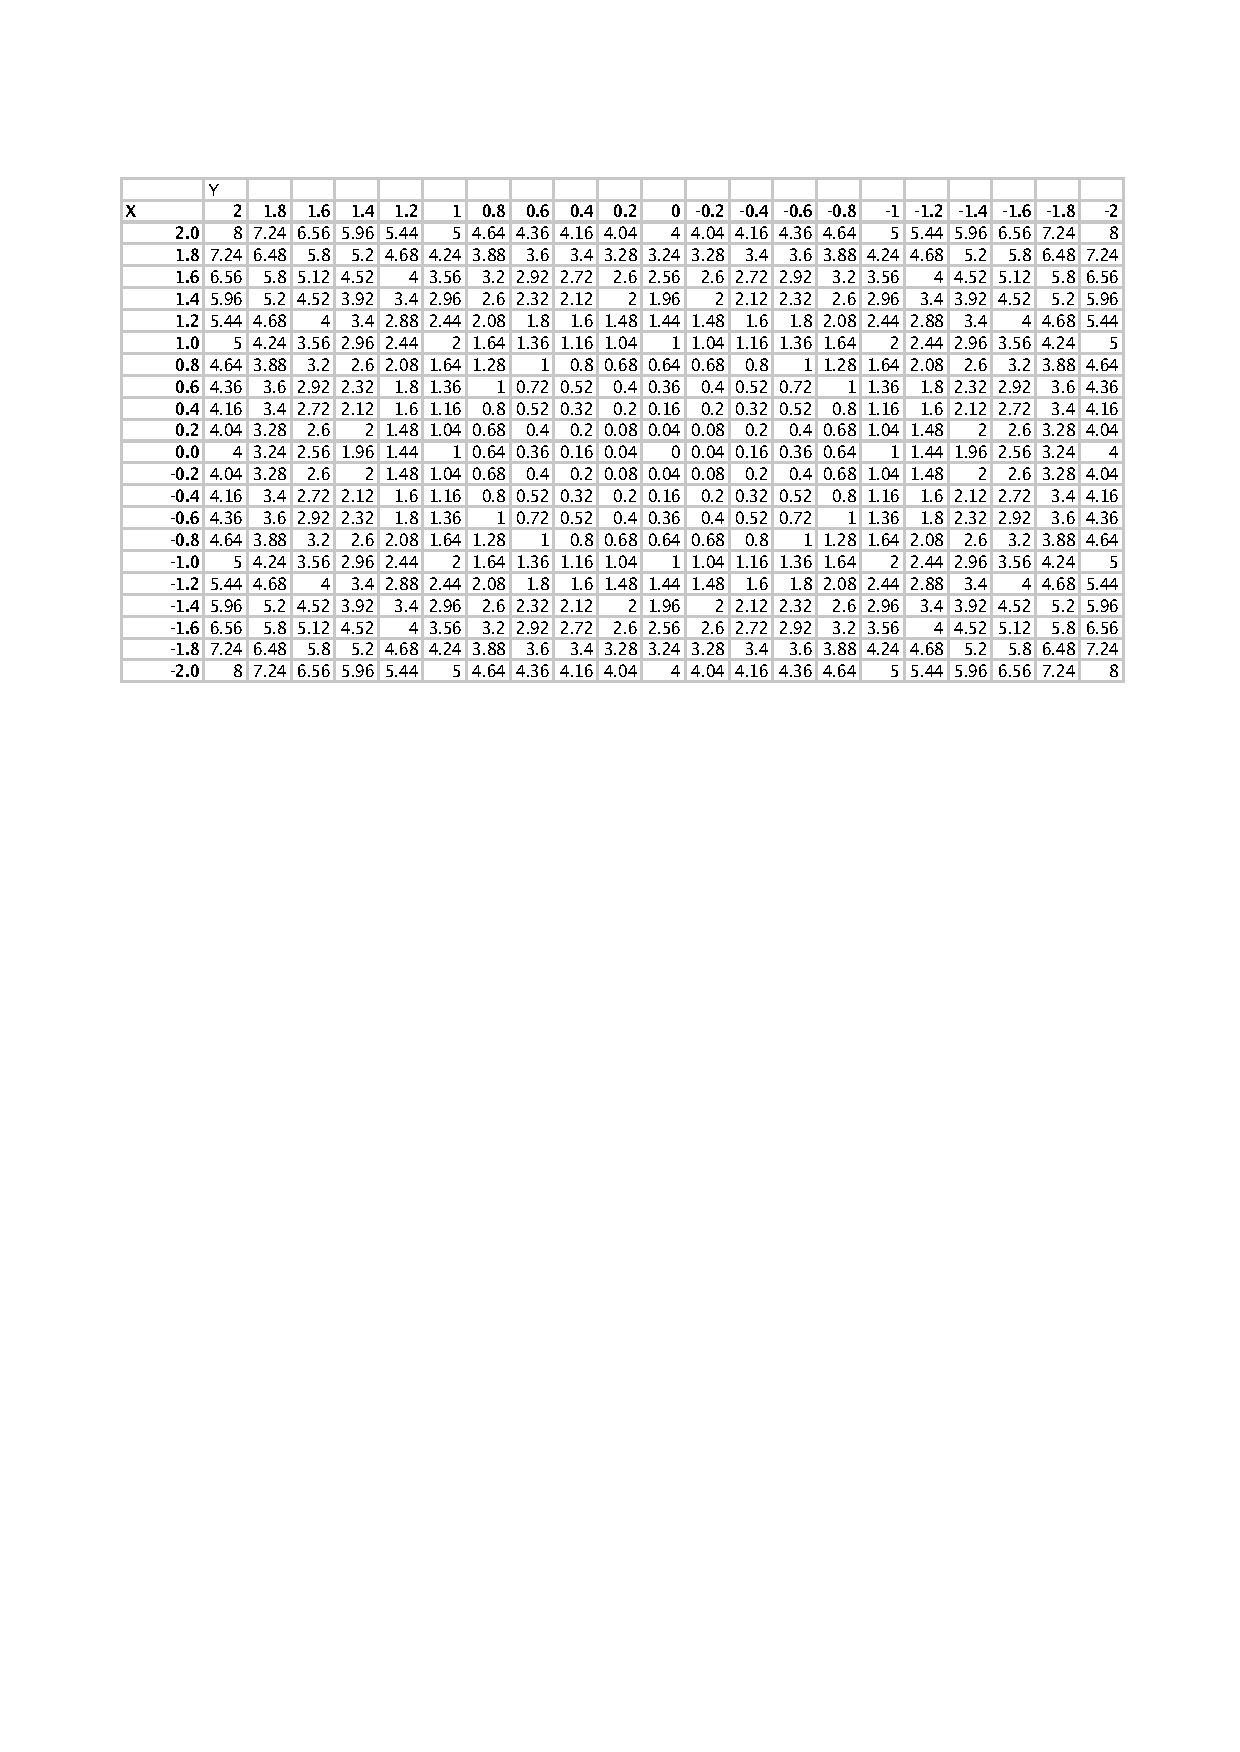
\includegraphics[width=5.0in]{table.jpg}
\vspace{-4mm}
\caption{Values for a linear function.}
\label{fig:table}
\end{center}
\end{figure}
\vspace{-7mm}

\item In Fig.~\ref{fig:table} is shown some values for a linear
  function.  Fill in the missing entries.



\item Consider the function $f(x,y) = 4 + x - 2y$.
\begin{enumerate}
\item Fill out a table of values for this function for $x$ and $y$
  from $-2$ to $2$, in increments of $1$.

\item Using your table of numbers, sketch the contour lines for this
  function.

\item Determine the contour lines using algebra.

\item Sketch $f(4,y)$.  What is the meaning of this function?

\item Sketch $f(x,4)$.  What is the meaning of this function?

\item Suppose you are standing at the origin on this surface.  What is
  your altitude?  In what direction would you have to walk to maintain
  your altitude?  In what direction is it the steepest up?  In what
  direction is it the steepest down?
\end{enumerate}


\item Consider a plane that passes through the points $(1,3,-2)$,
  $(-1,-3,4)$ and $(2,1,-2)$. 
\begin{enumerate}
  \item Determine the equation of this plane.
\item Sketch the contour lines for this plane.

\item Suppose you are standing at the point $x=1,y=2$.  What is your
  altitude?  In what direction would you need to walk to not change
  altitude?  In what direction is it the steepest up?  In what
  direction is it the steepest down?  Indicate these directions with
  arrows on your sketch.


\end{enumerate}
\end{enumerate}




\end{document}


 
